\documentclass[../main.tex]{subfiles}

\graphicspath{{pictures/}{../pictures/}}

\chapterimage{chapter_head_8.pdf} % Chapter heading image

\begin{document}
	%----------------------------------------------------------------------------------------
	%	Data Structures
	%----------------------------------------------------------------------------------------
	\chapter{Data Structures}
	As you've seen with C up until this point, you tend to have to build everything yourself.  This is why understanding data structures is an important skill to have.  In the following sections, we'll discuss \textit{linked-lists}, \textit{queues}, \textit{stacks}, \textit{binary search tree}, and \textit{hashtable}.  There are multiple ways that they could be constructed.  The following examples have been made to store data of type \textit{void *} so that they can be used with any data type.  An understanding of pointers and dynamic memory will be essential when building and working with custom data structures.
	
	\section{Linked-List}
	A \textit{linked-list} is a fairly simple data structure where one node points to the next node.  You may see a \textit{singly linked-list}, \textit{doubly linked-list}, and even a \textit{circly linked-list}.  We'll keep it simple with a \textit{singly linked-list}.\\
	
	\lstinputlisting[caption={\lstname}, label={lst:ll_header}]{src/09-ll.h}
	In the header file we have two \textit{structs}, \textit{ll\_t} and \textit{node\_t}.  The \textit{ll\_t struct} will contain the first \textit{node\_t} which is called the "head".  The "next" pointer in each \textit{node\_t struct} will point to the next node in the list unless there are no additional nodes.  In that case, the "next" pointer will be \textit{NULL}.
	
	\begin{figure}[h]
		\centering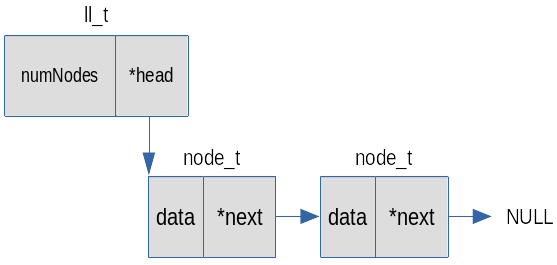
\includegraphics[scale=0.5]{linkedlist.png}
		\caption{Linked-List}
		\label{fig:linked_list}
	\end{figure}

	\lstinputlisting[caption={\lstname}, label={lst:ll}]{src/09-ll.c}
	
	\section{Queue}
	
	\lstinputlisting[caption={\lstname}, label={lst:queue_header}]{src/09-queue.h}
	\lstinputlisting[caption={\lstname}, label={lst:queue}]{src/09-queue.c}
	
	\section{Stack}
	
	\lstinputlisting[caption={\lstname}, label={lst:stack_header}]{src/09-stack.h}
	\lstinputlisting[caption={\lstname}, label={lst:stack}]{src/09-stack.c}
	
	\section{Binary Search Tree}
	
	\section{HashTable}
	
\end{document}